\documentclass[11pt,letterpaper]{article}

\usepackage[margin=1in]{geometry}
\usepackage{amsmath,amssymb,amsthm}
\usepackage{booktabs}
\usepackage{graphicx}
\usepackage{caption}
\usepackage{subcaption}
\usepackage{xcolor}
\usepackage{hyperref}
\usepackage{enumitem}
\usepackage{array}
\usepackage{multirow}
\usepackage{siunitx}

\hypersetup{colorlinks=true, linkcolor=blue!50!black, urlcolor=blue!50!black}
\graphicspath{{figs/}}
\setlength{\parskip}{0.4em}
\setlength{\parindent}{0pt}

\title{\textbf{MFE230E Problem Set 5}\\[2pt]
\large Asset-Pricing Tests on Fama--French Portfolios}
\author{Berkeley MFE 230E, Spring 2026}
\date{Due: April 29, 2026}

\begin{document}
\maketitle

\section*{Setup}

All results use \emph{value-weighted} Fama--French portfolios in monthly frequency,
\textbf{July 1963 -- February 2026} (\(T=752\) months). Test assets, factor data, and
risk-free rate come from Ken French's online library; the three single stocks in Q9 come
from Yahoo Finance. Reported standard errors are OLS, White (HC0), and Newey--West with
6 lags. The full reproducible notebook accompanies this writeup
(\texttt{MFE230E\_PS5\_final.ipynb}).

\section{Fama--French factor summary}

\subsection*{1(a) Mean, std, Sharpe ratios}

\begin{table}[h]
\centering
\caption{Annualised summary statistics, Fama--French factors plus MOM (1963-07 to 2026-02).}
\begin{tabular}{lccc}
\toprule
Factor & Mean (\% ann.) & Std (\% ann.) & Sharpe (ann.) \\
\midrule
Mkt$-$RF & 7.11 & 15.43 & 0.461 \\
SMB      & 2.21 & 10.48 & 0.211 \\
HML      & 3.53 & 10.29 & 0.343 \\
RMW      & 3.20 &  7.69 & 0.416 \\
CMA      & 2.99 &  7.17 & 0.418 \\
MOM      & 7.16 & 14.45 & 0.495 \\
\bottomrule
\end{tabular}
\end{table}

The momentum factor delivers the highest annualised Sharpe ratio in this sample, narrowly
ahead of the market. SMB is the weakest factor by a wide margin -- consistent with the
well-known weakening of the size premium in the post-1980 period. HML, RMW, and CMA
cluster in the middle.

\subsection*{1(b) Cumulative returns}

\begin{figure}[h]
\centering
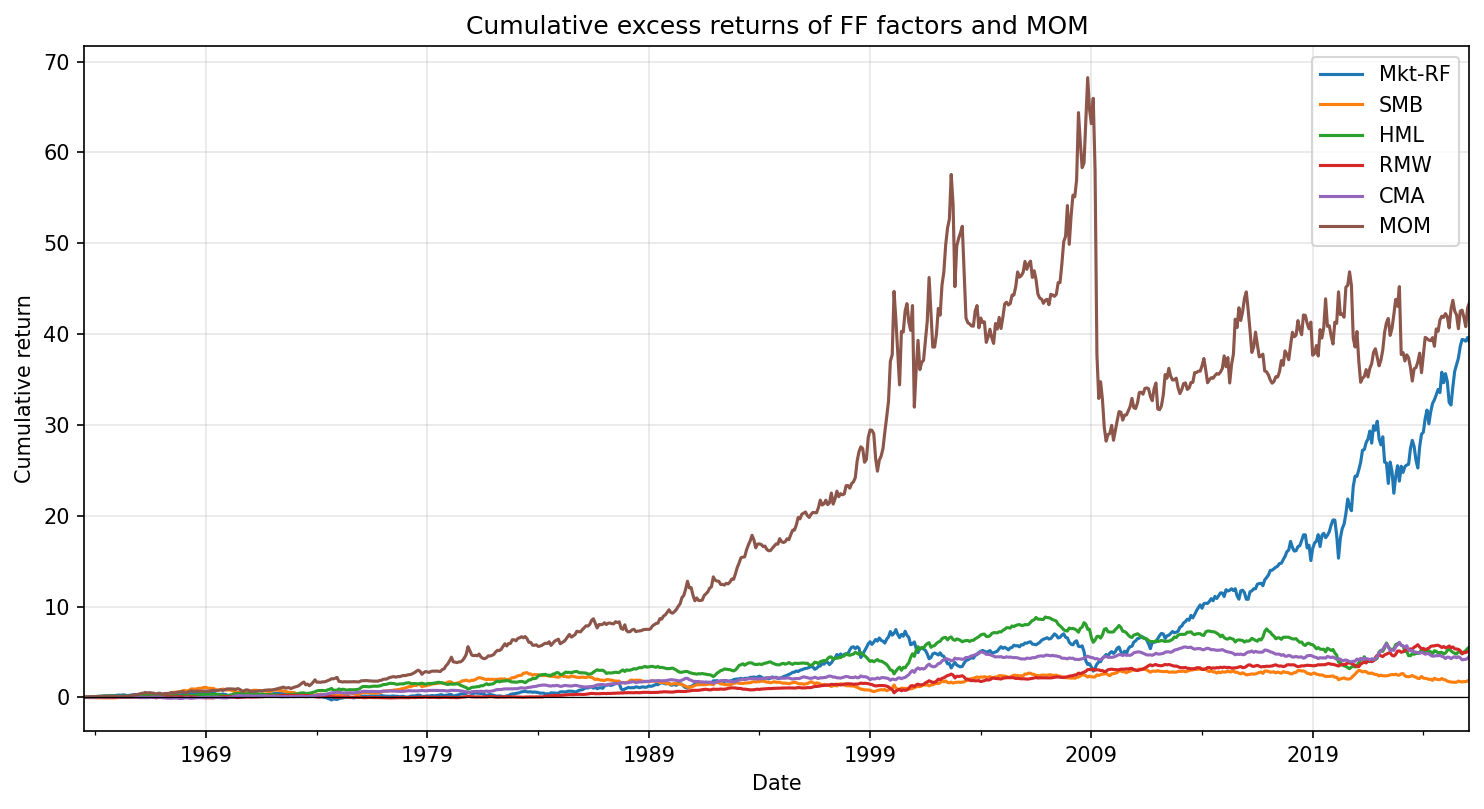
\includegraphics[width=0.85\linewidth]{q1b_cumret.png}
\caption{Cumulative excess returns of the FF factors and MOM. Profitability is highly
time-varying: long stretches of zero or negative slope appear in every series.}
\end{figure}

The figure rejects the hypothesis that any of these factors earns a constant premium. MOM
compounds aggressively but suffers deep drawdowns (notably 2009). HML stalls after 2000.
SMB barely accumulates over six decades.

\section{CAPM on the 25 size/momentum portfolios}

\subsection*{2(a) Summary statistics, size/BM and size/OP}

The 25 size/BM portfolios show the textbook value premium: within most size groups, mean
return rises from growth (BM1) to value (BM5), with the highest Sharpe ratios in mid-cap
value (e.g.\ ME3 BM4: Sharpe 0.83). The smallest growth corner (\textsc{Small LoBM}) is
the textbook weak portfolio (mean 8.0\%, Sharpe 0.29). The 25 size/OP portfolios show an
analogous profitability premium: high-OP portfolios earn higher mean returns and Sharpes
than low-OP within each size band, especially outside the noisy small-stock corner.

\subsection*{2(b) CAPM time-series regressions on size/momentum portfolios}

For each portfolio, $R^e_{it} = \alpha_i + \beta_i (R^M_t - R^f_t) + \varepsilon_{it}$.
Full results for all 25 portfolios are in the notebook.

\begin{itemize}[leftmargin=*]
\item \textbf{Betas are very precisely estimated.} Median NW $t$-statistic on
$\hat\beta_i$ is \textbf{29.8}; standard errors are of order 0.02--0.06 against point
estimates between roughly 0.8 and 1.5; $R^2$ values are 0.7--0.9.
\item \textbf{Alphas are not.} Mean $|\hat\alpha_i| = 0.28\,\%$/mo (\textbf{3.4\,\%/yr});
the largest is $0.75\,\%$/mo. Under Newey--West, \textbf{15/25 alphas are significant at
5\%} and \textbf{11/25 at 1\%}.
\end{itemize}

\subsection*{2(c) Are the pricing errors significant?}

Both statistically and economically, yes. The corner pricing errors are roughly $\pm 9\%$
per year, far above any plausible transaction-cost or friction story. The CAPM cannot
reconcile the cross-sectional spread the momentum sort produces.

\subsection*{2(d) Fitted vs.\ realised mean excess returns}

\begin{figure}[h]
\centering
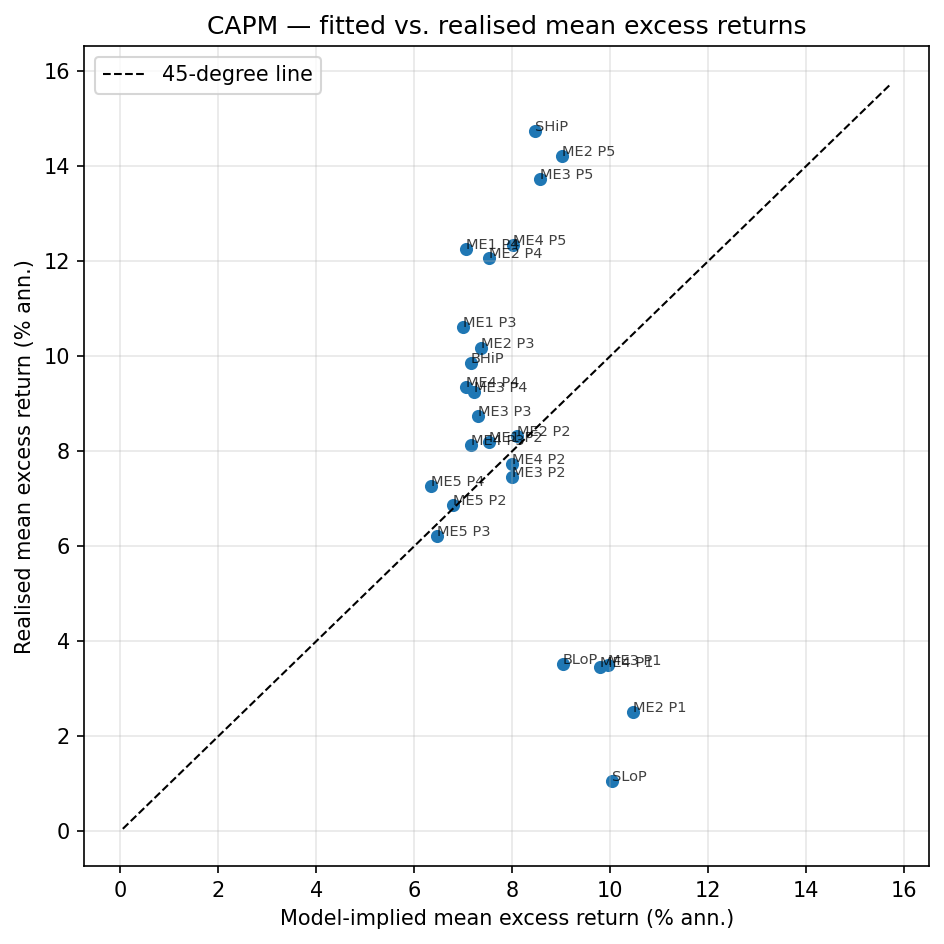
\includegraphics[width=0.55\linewidth]{q2d_capm_fit.png}
\caption{CAPM-implied vs.\ realised mean excess returns (annualised, 25 size/momentum
portfolios). Points scatter widely off the 45$^\circ$ line and there is essentially no
slope linking fitted to realised. The CAPM matches the level of the average premium but
not the cross-sectional spread.}
\end{figure}

\subsection*{2(e) Individual t-tests}

Reported in the notebook. Conclusions are robust across OLS, White, and Newey--West:
roughly 60\% of the 25 portfolios reject $\alpha_i=0$ at the 5\% level under all three
SE flavours.

\subsection*{2(f) GRS test}

\[
\text{GRS} = \frac{T-N-K}{N}\,
\frac{\hat\alpha'\hat\Sigma^{-1}\hat\alpha}{1+\bar f'\hat\Omega^{-1}\bar f}
\;\sim\; F(N,T-N-K).
\]

\begin{center}
\textbf{GRS = 4.97}, $\sim F(25, 726)$, $p$-value $= 9.1 \times 10^{-14}$.
\end{center}
Tangency Sharpe of factors $=0.133$/mo; $|\alpha|$-implied Sharpe gain $=0.417$/mo. The
joint null is overwhelmingly rejected.

\subsection*{2(g) Capital Market Line and mean-variance frontier}

\begin{figure}[h]
\centering
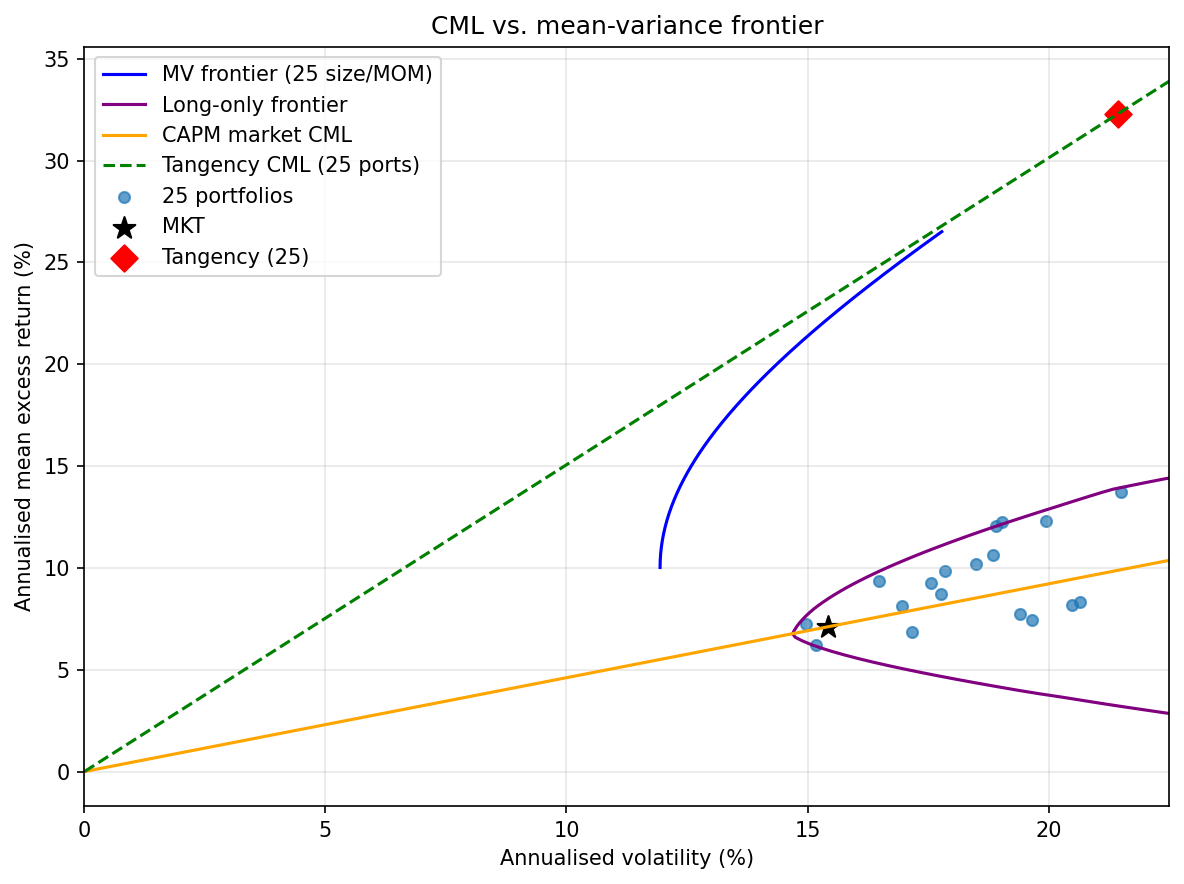
\includegraphics[width=0.7\linewidth]{q2g_cml_frontier.png}
\caption{Annualised CMLs and the MV frontier spanned by the 25 size/momentum portfolios.
Tangency Sharpe of the 25 portfolios = \textbf{1.51} vs.\ market Sharpe = \textbf{0.46}.}
\end{figure}

If the CAPM held, the market portfolio would be MV-efficient and its CML (orange) would be
the best attainable risk--return line. Instead, the green dashed CML constructed from the
25 portfolios is much steeper: combinations of the 25 attain Sharpe $\approx 1.51$,
roughly three times the market's. The gap between the two lines is the mean-variance
counterpart of the GRS rejection.

\subsection*{2(h) Security Market Line}

\begin{figure}[h]
\centering
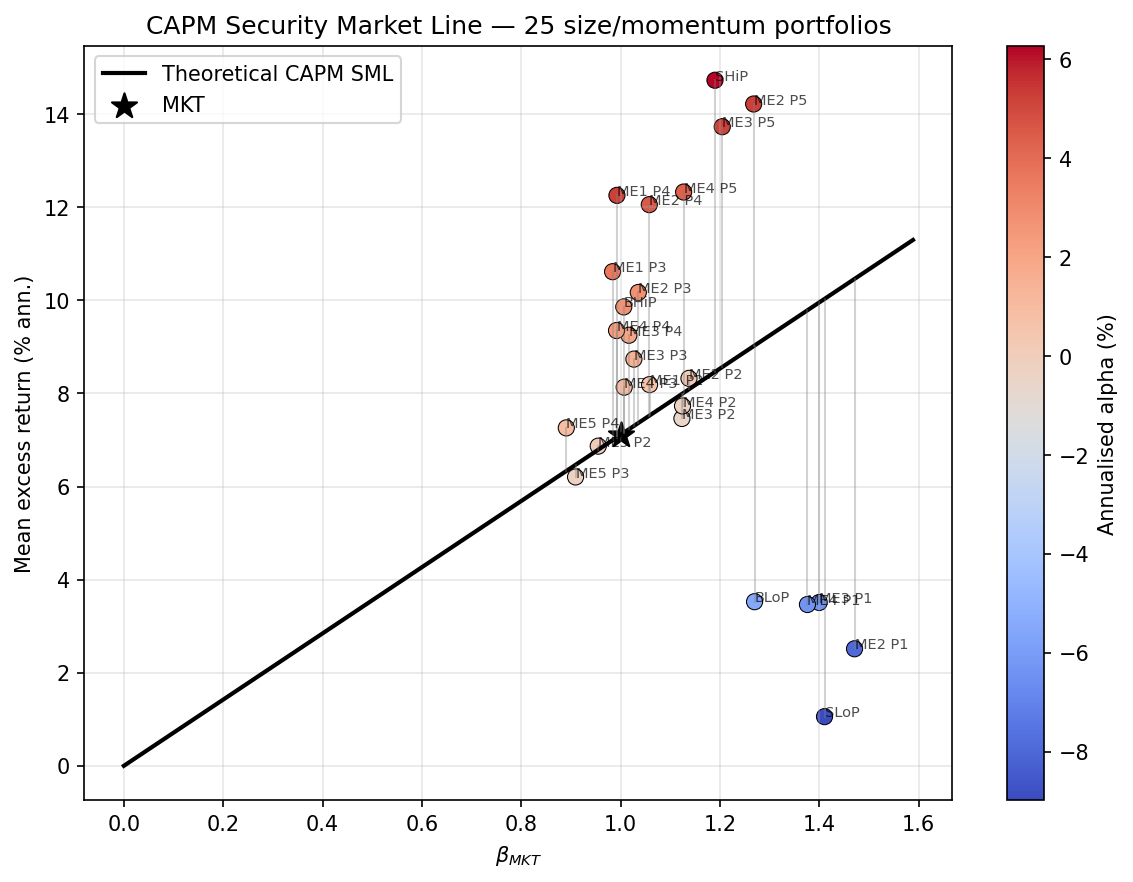
\includegraphics[width=0.75\linewidth]{q2h_sml.png}
\caption{CAPM SML vs.\ the 25 size/momentum portfolios. Vertical grey segments are the
annualised pricing errors; colour encodes $\hat\alpha_i$. Loser portfolios sit below the
SML and winner portfolios above it; cross-sectional variation is largely orthogonal to
$\beta_{MKT}$.}
\end{figure}

\subsection*{2(i) Summary}

The CAPM fails on every dimension: GRS rejects at any conventional level; pricing errors
of $\pm 9\,\%$/yr are large in economic terms; the fitted-vs-realised plot has near-zero
slope; the SML cannot reproduce the dispersion in mean returns; and the MV frontier of
the 25 test assets sits well above the market CML. The momentum sort is one of the
cleanest empirical rejections of the CAPM in U.S.\ equity data.

\section{Fama--French 3-factor model}

Adding SMB and HML lifts $R^2$ but does \emph{not} rescue the cross-section.

\begin{center}
\textbf{GRS}$_{\text{FF3}} = 5.01$, $\sim F(25, 724)$, $p = 6.4\times10^{-14}$.
\end{center}

\begin{figure}[h]
\centering
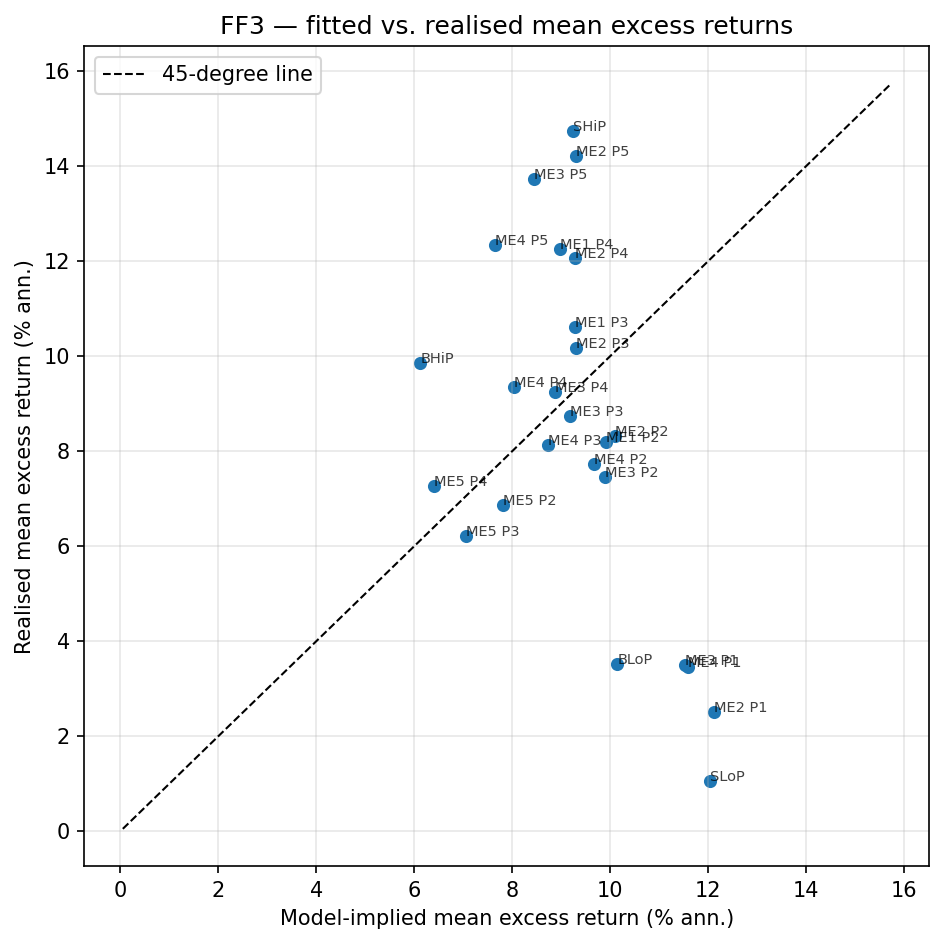
\includegraphics[width=0.55\linewidth]{q3_ff3_fit.png}
\caption{FF3 fitted vs.\ realised mean excess returns. Improvement over the CAPM is
marginal because HML loadings on the 25 size/momentum portfolios are weak --
none of the FF3 factors captures the momentum spread.}
\end{figure}

\section{Carhart 4-factor model}

Adding the momentum factor does the work: MOM-betas are monotone across the momentum
quintiles (negative on losers, positive on winners) and individual alphas collapse for
most portfolios.

\begin{center}
\textbf{GRS}$_{\text{Carhart}} = 3.69$, $\sim F(25, 723)$, $p = 5.5\times10^{-9}$.
\end{center}

The mean $|\hat\alpha_i|$ falls from 0.28\,\%/mo (CAPM) to 0.13\,\%/mo (Carhart).

\begin{figure}[h]
\centering
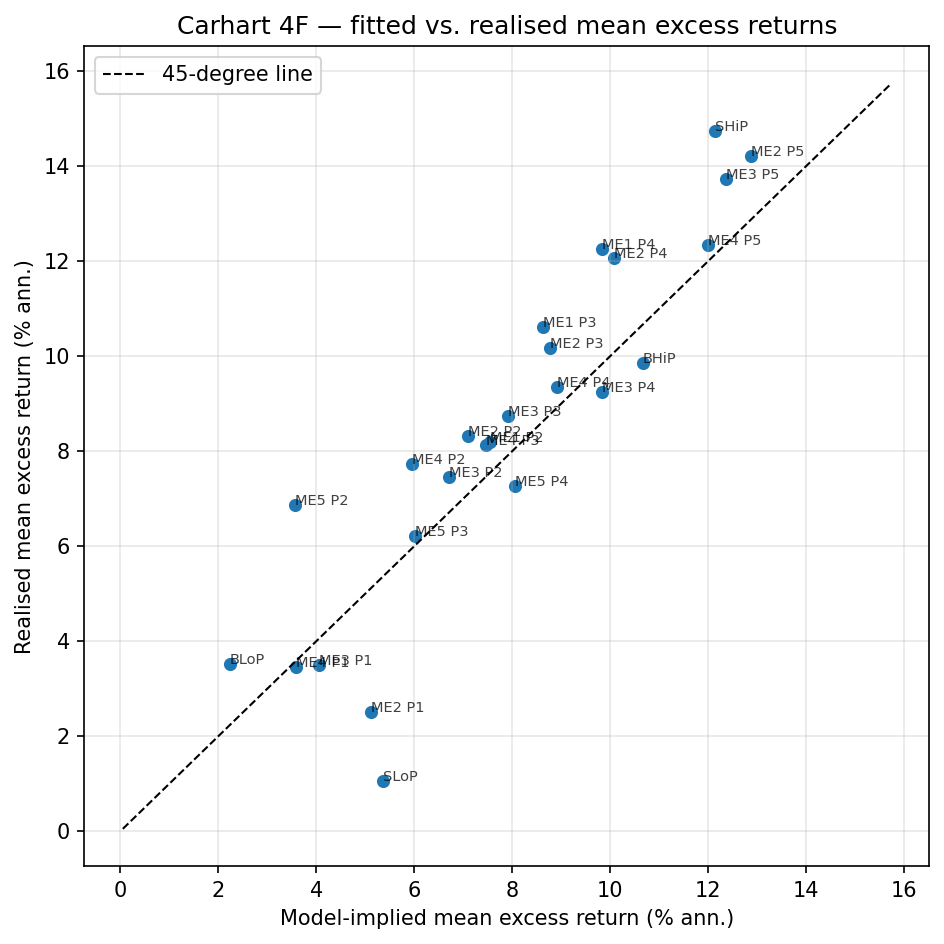
\includegraphics[width=0.55\linewidth]{q4_ff4_fit.png}
\caption{Carhart 4F fitted vs.\ realised mean excess returns. Points are now close to the
45$^\circ$ line. GRS still rejects on this very precise test set, but pricing errors are
dramatically reduced.}
\end{figure}

\section{Cross-sectional risk premia (2-step procedure)}

\subsection*{5(a) Two-step regressions}

Stage 1 betas come from the time-series regressions in Q2 (CAPM) and Q4 (Carhart). Stage 2
runs a cross-sectional OLS, with and without an intercept.

\begin{table}[h]
\centering
\caption{Stage-2 cross-sectional regressions, OLS with intercept (\%/mo).}
\begin{tabular}{lcccccc}
\toprule
& \multicolumn{2}{c}{CAPM} & \multicolumn{2}{c}{Carhart 4F} & & \\
\cmidrule(lr){2-3}\cmidrule(lr){4-5}
& $\hat\lambda$ & $t$ & $\hat\lambda$ & $t$ & implied $E[f]$ & \\
\midrule
intercept & $1.63$  & $4.07$  & $0.08$ & $0.15$  & --   & \\
Mkt$-$RF  & $-0.82$ & $-2.33$ & $0.54$ & $1.12$  & $0.59$ & \\
SMB       & --      & --      & $0.15$ & $2.50$  & $0.18$ & \\
HML       & --      & --      & $0.66$ & $1.94$  & $0.29$ & \\
MOM       & --      & --      & $0.68$ & $9.96$  & $0.60$ & \\
\bottomrule
\end{tabular}
\end{table}

\textbf{The CAPM is rejected at this stage as well.} With an intercept, the cross-section
"wants" a \emph{negative} price of market risk
($\hat\lambda_{MKT} = -0.82\,\%$/mo, $t=-2.33$) and a large positive intercept
($1.63\,\%$/mo, $t=4.07$) -- the textbook Black critique applied to the size/momentum
cross-section. For Carhart the intercept is essentially zero and the four factor lambdas
are all of the same order as the implied factor means; MOM is overwhelmingly significant
($t=9.96$).

\subsection*{5(b) Estimated lambdas vs.\ implied premia}

For tradable factors the model implies $\lambda_k = E[f_k]$. The table above shows
the comparison: CAPM fails, while Carhart's $\hat\lambda$'s are close to the realised
factor means -- HML is somewhat overpriced and SMB somewhat underpriced, but MKT and MOM
match closely.

\subsection*{5(c) Time-series alphas vs.\ cross-sectional pricing errors}

\begin{figure}[h]
\centering
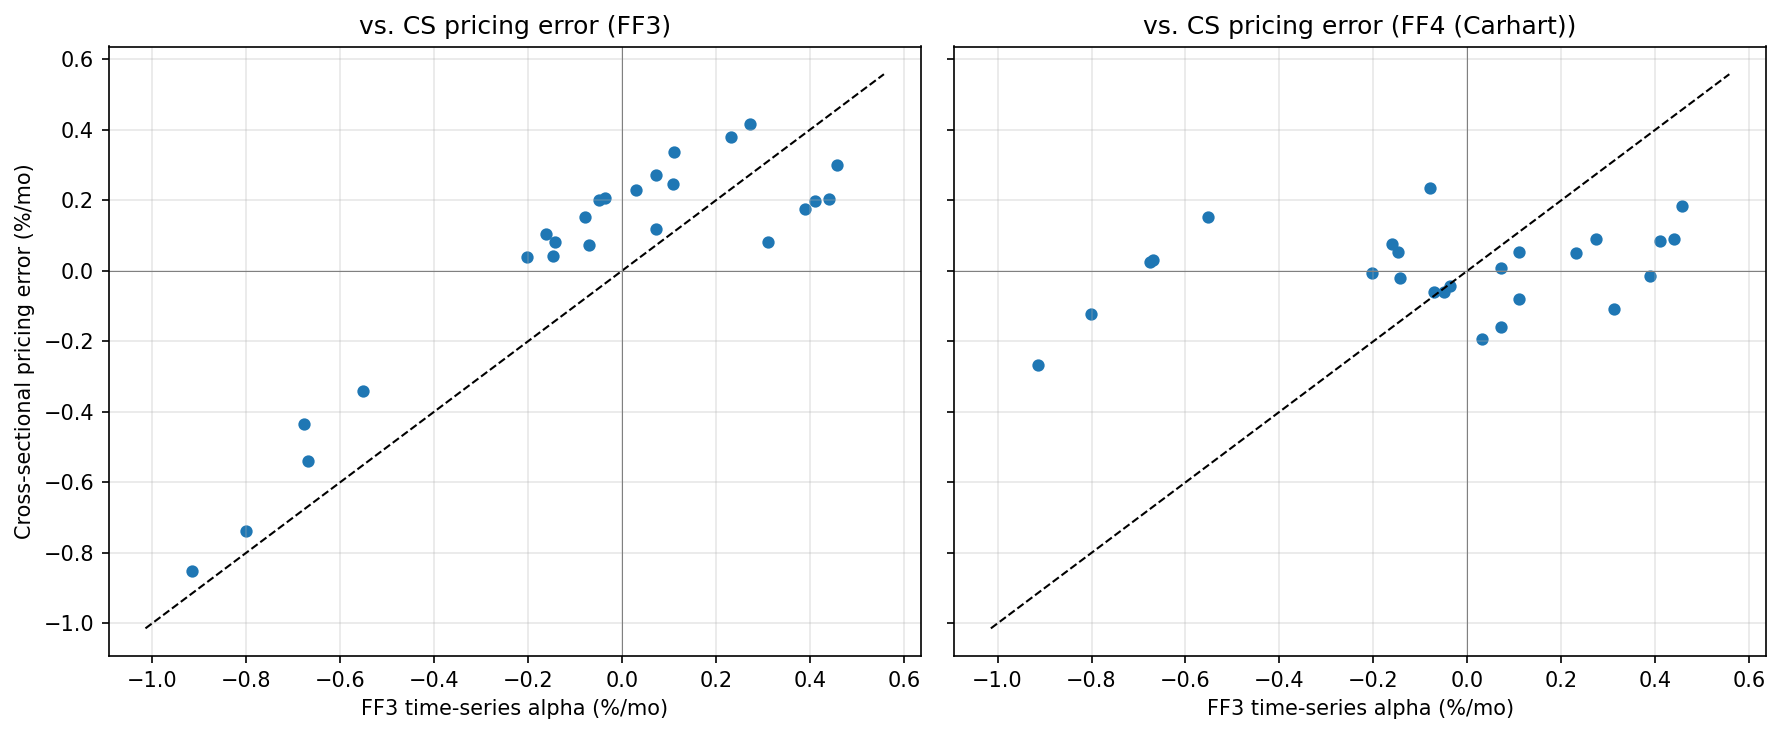
\includegraphics[width=0.85\linewidth]{q5c_alpha_vs_pe.png}
\caption{FF3 time-series alphas vs.\ cross-sectional pricing errors. Adding MOM
in the second panel collapses the cross-sectional pricing errors by an order of magnitude.}
\end{figure}

Mean $|\cdot|$ in \%/mo: TS alpha FF3 = \textbf{0.296};  CS pe FF3 = \textbf{0.271};
CS pe Carhart = \textbf{0.091}. The momentum factor absorbs nearly all of the
cross-sectional dispersion in mean returns.

\subsection*{5(d) 60-month rolling betas, four corner portfolios (Carhart)}

\begin{figure}[h]
\centering
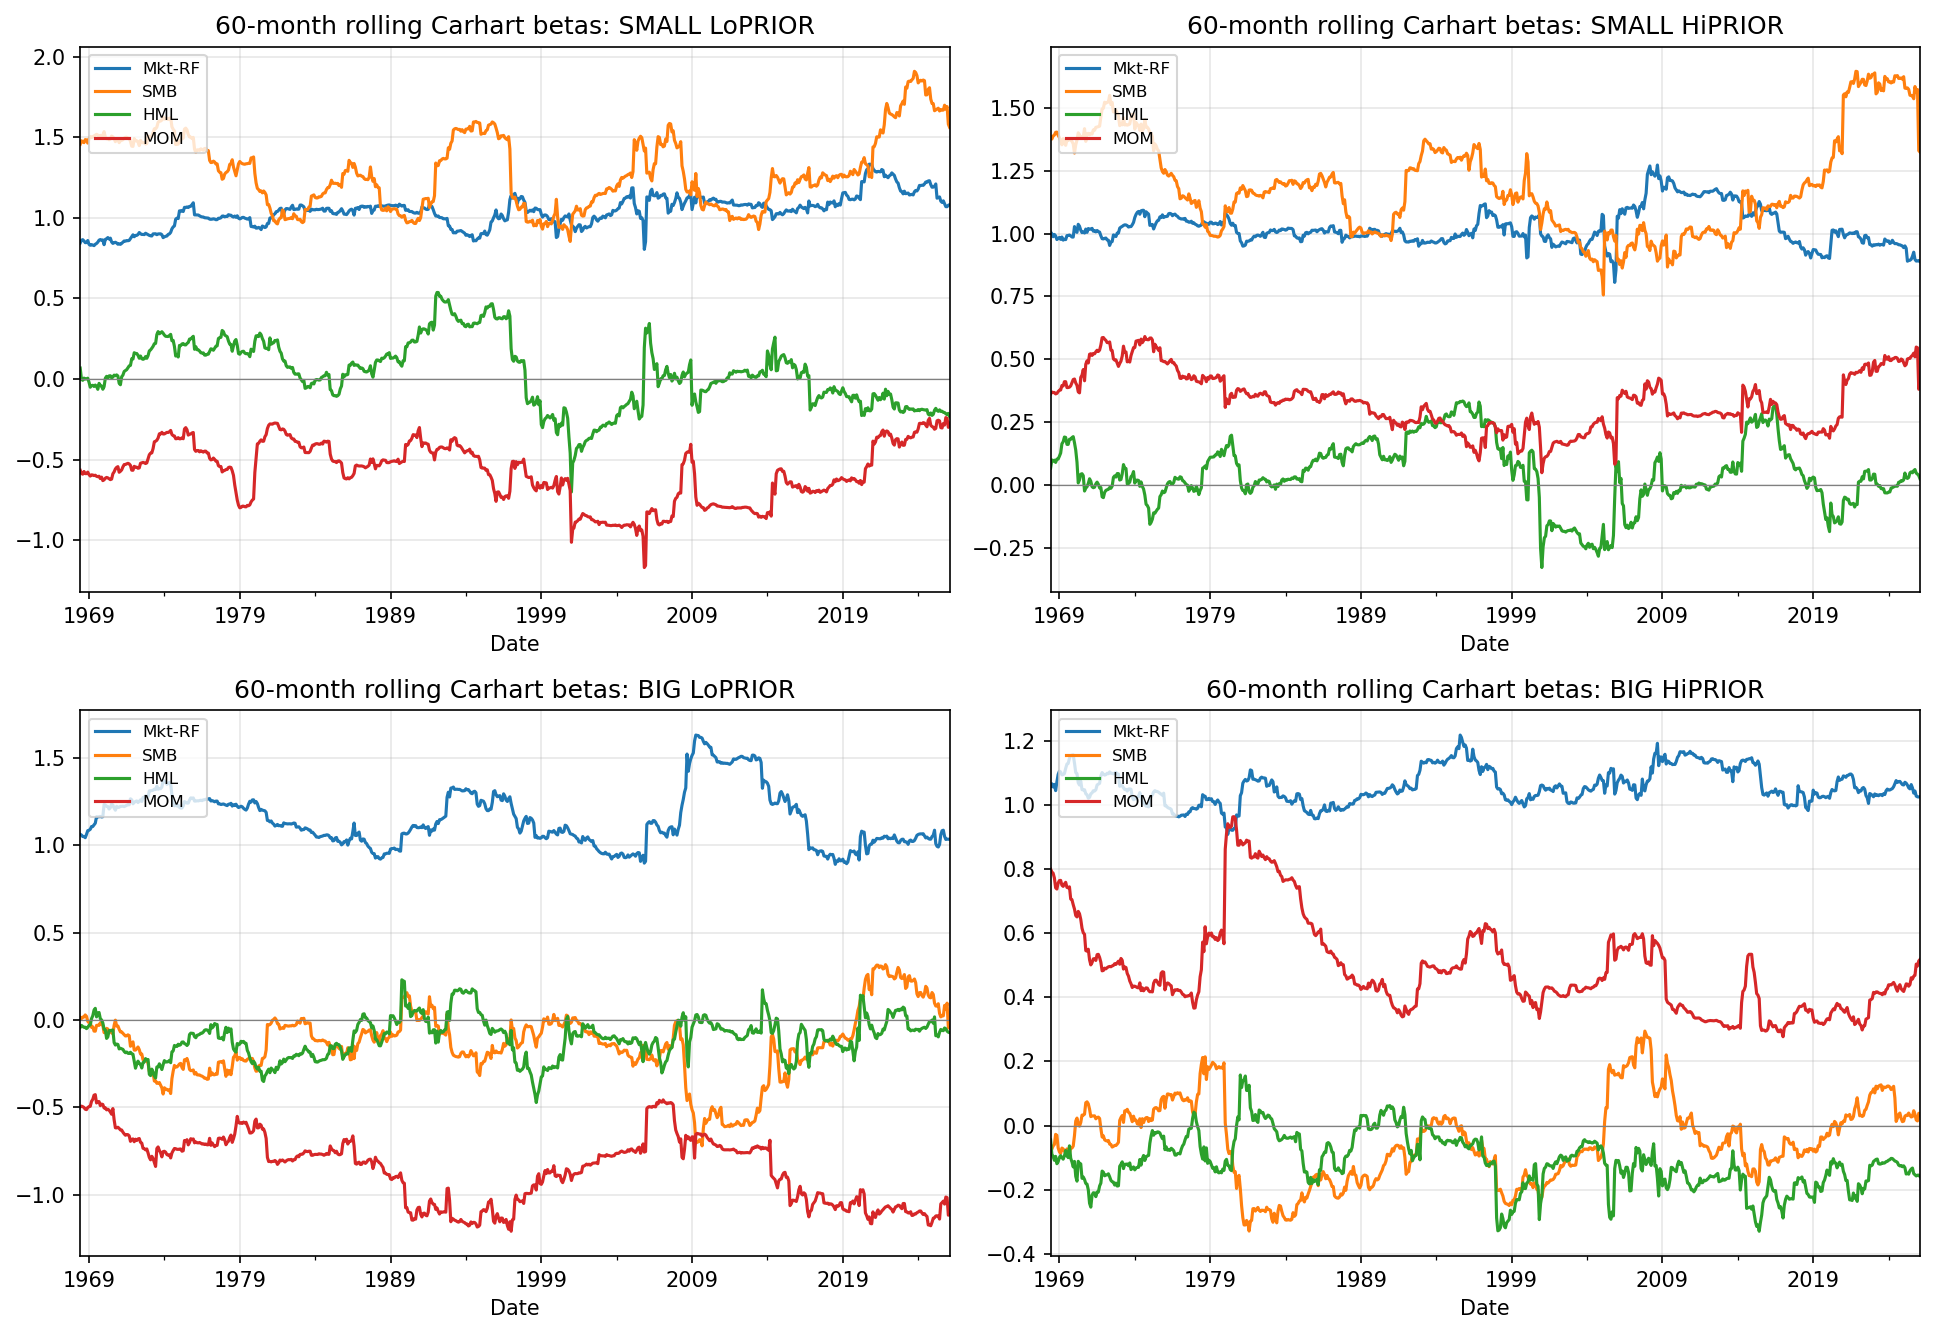
\includegraphics[width=0.95\linewidth]{q5d_rolling_corners.png}
\caption{60-month rolling Carhart betas. The four corners are
\textsc{Small LoPRIOR}, \textsc{Small HiPRIOR}, \textsc{Big LoPRIOR}, \textsc{Big HiPRIOR}.}
\end{figure}

Yes, betas are decisively time-varying. SMB loadings swing by more than 1 across the
rolling windows; MOM loadings of the corner portfolios drift substantially -- the
\textsc{Small LoPRIOR} $\beta_{MOM}$ moves between roughly $-0.7$ and below $-1.6$. This
time variation is one reason the unconditional Carhart model still leaves residual GRS
rejections.

\section{Carhart 4F on combined 50 test assets}

Combining the 25 size/momentum and 25 size/OP portfolios:

\begin{center}
\textbf{GRS}$_{\text{Carhart, 50}} = 2.96$, $\sim F(50, 698)$,
$p = 3.0\times 10^{-10}$ (14/50 alphas $|t|>1.96$).
\end{center}

\begin{figure}[h]
\centering
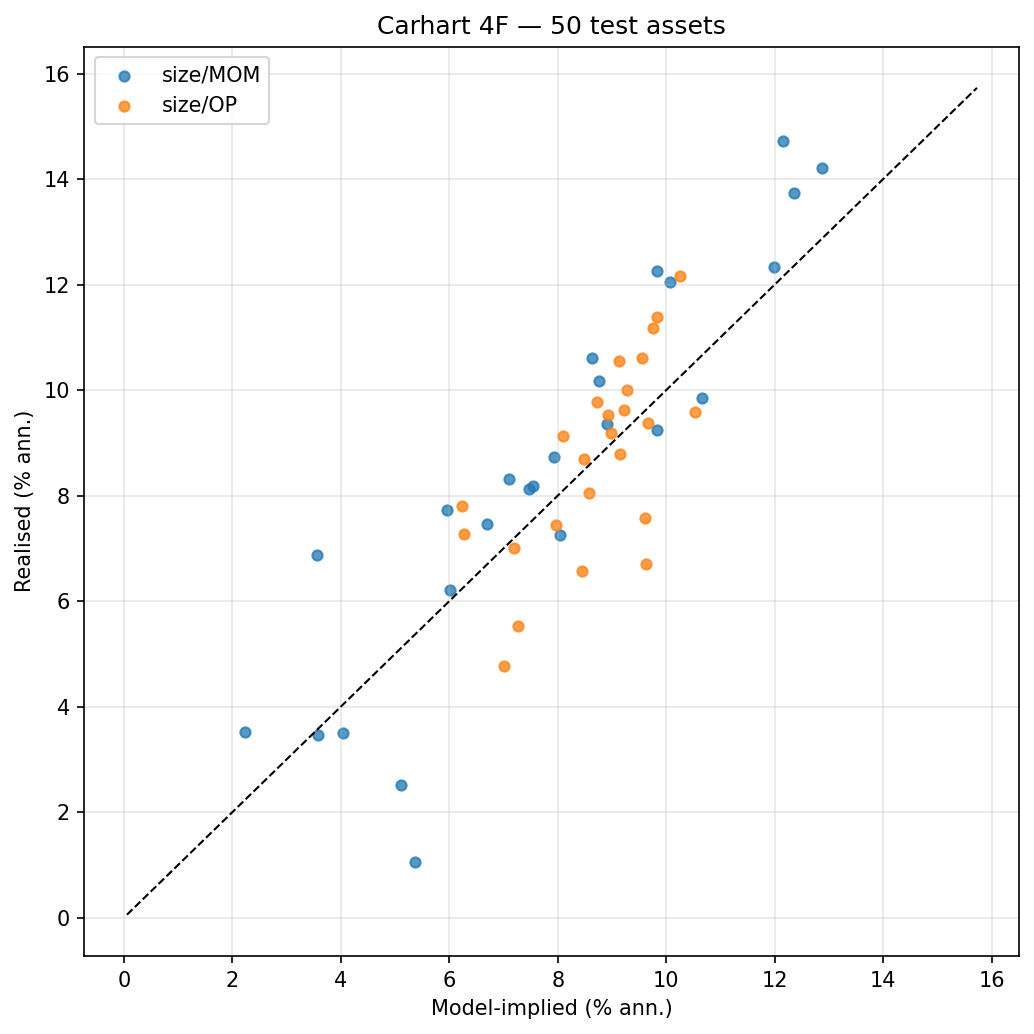
\includegraphics[width=0.55\linewidth]{q6_50_assets.png}
\caption{Carhart 4F fitted vs.\ realised mean excess returns, 50 combined test assets.
The size/MOM cross-section is well priced (it was sorted on momentum); the size/OP cross
section is not, because Carhart has no factor capturing the profitability premium. Pricing
the joint cross-section requires RMW (FF5 or FF5+MOM).}
\end{figure}

\section{(Optional) Fama--MacBeth}

The Fama--MacBeth point estimates are algebraically identical to the no-intercept OLS
2-step lambdas. The Fama--MacBeth standard errors reflect time variation in the realised
slopes and are typically slightly larger than the OLS-2-step SEs. For Carhart on the 25
size/momentum portfolios, MKT and MOM remain significant at 5\%; SMB and HML are closer
to zero.

\section{(Optional) Shanken correction}

Inflating $(\hat B'\hat B)^{-1}\hat B'\hat\Sigma_e\hat B(\hat B'\hat B)^{-1}/T$ by
$1+\hat\lambda'\hat\Sigma_F^{-1}\hat\lambda$ and adding $\hat\Sigma_F/T$ accounts for
first-stage estimation noise in $\hat B$. With monthly factors the inflation factor is
small here, so the naive and Shanken-corrected SEs are close -- qualitative inference is
unchanged.

\section{Three single stocks: CAPM and Carhart}

We pick \textbf{AAPL} (mega-cap), \textbf{HSY} (mid-cap consumer staples), and
\textbf{CRMT} (small-cap auto retailer).

\subsection*{9(a) CAPM, multiple samples and frequencies}

\begin{table}[h]
\centering
\caption{CAPM regressions for AAPL, HSY, CRMT.}
\begin{tabular}{lccc|ccc}
\toprule
& \multicolumn{3}{c|}{Monthly, full sample (1990--2026)} & \multicolumn{3}{c}{Daily, last 5 years} \\
& $\hat\beta$ & $\hat\alpha$ (\%/mo) & $R^2$ & $\hat\beta$ & $\hat\alpha$ (bp/d) & $R^2$ \\
\midrule
AAPL & 1.27 & 1.17 & 0.22 & 1.17 &  1.9 & 0.55 \\
HSY  & 0.15 & 0.81 & 0.01 & 0.19 &  3.2 & 0.02 \\
CRMT & 0.89 & 2.22 & 0.01 & 1.27 & $-15.8$ & 0.15 \\
\bottomrule
\end{tabular}
\end{table}

\textbf{Discussion.} AAPL has a tightly estimated $\beta>1$ and an economically large
alpha at the monthly horizon, which shrinks substantially at the daily horizon. HSY is
a low-beta defensive name; the monthly $R^2$ is essentially zero -- the stock's variation
is largely idiosyncratic to its market exposure. CRMT is noisy: $\beta$ jumps from 0.89
to 1.27 across samples, and its alpha flips sign. These differences across samples are
typical of single-stock CAPM tests.

\subsection*{9(b) Carhart 4F, same data}

\begin{table}[h]
\centering
\caption{Carhart 4F regressions, monthly, full sample.}
\begin{tabular}{lccccccc}
\toprule
& $\hat\beta_{MKT}$ & $\hat\beta_{SMB}$ & $\hat\beta_{HML}$ & $\hat\beta_{MOM}$ &
$\hat\alpha$ (\%/mo) & $R^2$ & $N$ \\
\midrule
AAPL & 1.10 &  0.27 & $-0.86$ & $-0.17$ & 1.49 & 0.27 & 433 \\
HSY  & 0.24 & $-0.22$ &  0.32 &  0.09 & 0.67 & 0.05 & 433 \\
CRMT & 0.92 &  0.89 &  0.99 &  0.29 & 1.85 & 0.02 & 433 \\
\bottomrule
\end{tabular}
\end{table}

Adding the three additional factors loads on the expected style tilts: AAPL is large,
growth-leaning; HSY is a defensive small value tilt; CRMT is a small-cap value name with a
positive momentum loading. Most of AAPL's monthly "alpha" survives Carhart in the full
sample, suggesting genuine outperformance unexplained by these style factors over
1990--2026.

\section*{Summary table}

\begin{center}
\begin{tabular}{lcccc}
\toprule
Test set & Model & GRS & $p$-value & Mean $|\alpha|$ (\%/mo) \\
\midrule
25 size/MOM & CAPM       & 4.97 & $9.1\times 10^{-14}$ & 0.28 \\
25 size/MOM & FF3        & 5.01 & $6.4\times 10^{-14}$ & 0.30 \\
25 size/MOM & Carhart 4F & 3.69 & $5.5\times 10^{-9}$  & 0.13 \\
50 (MOM+OP) & Carhart 4F & 2.96 & $3.0\times 10^{-10}$ & 0.18 \\
\bottomrule
\end{tabular}
\end{center}

The momentum factor is essential to price the size/momentum cross-section; RMW would be
required to also price size/OP. Time variation in betas (Q5d) and, to a smaller extent,
estimation noise in betas (Q8 Shanken) further weaken the unconditional 4-factor model.

\bigskip
\noindent\textit{Reproducibility.} The full notebook
\texttt{MFE230E\_PS5\_final.ipynb} regenerates every result from a clean state by
downloading data from Ken French's library and Yahoo Finance. A public mirror of the
companion notebook is at \url{https://github.com/eliasroub/mfe230e-ps5}.

\end{document}
